\chapter{Results}

\section{Intensity of Single Source - Diffraction}

Using python, I plotted distance vs. intensity for a single source. The relevant python code can be found in appendix \ref{code:single}.

\begin{figure}[!h]
\centering	
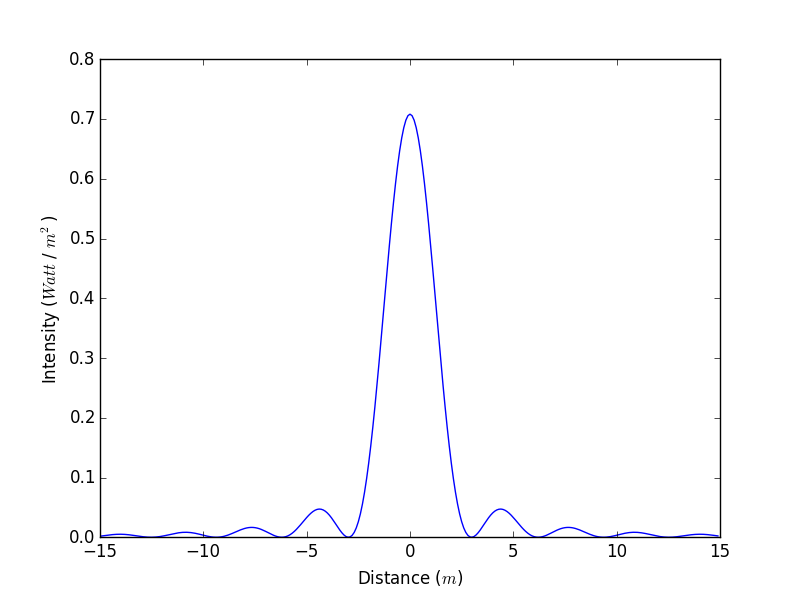
\includegraphics[scale=0.45]{figure_1.png}
\caption{Intensity profile of single antenna}
\end{figure}

\subsection{Discussion}
Here we have a single isotropic antenna source, radiating over a sphere centered on the source. It's intensity decreases by increasing the distance as it should be, because we have a spherical wave moving radially and with the passage of time when it cover some distance, it's intensity goes down and down. Where at the position where source is placed we have high intensity peak.


\section{Intensity of Linear Array of 4 Antennae}

Plot between distance and intensity, for four antenna sources arrange in a linear array and by introducing phase between them, we get interference pattern. The relevant code can be found in appendix \ref{code:four}.

\begin{figure}[!h]
	\centering	
    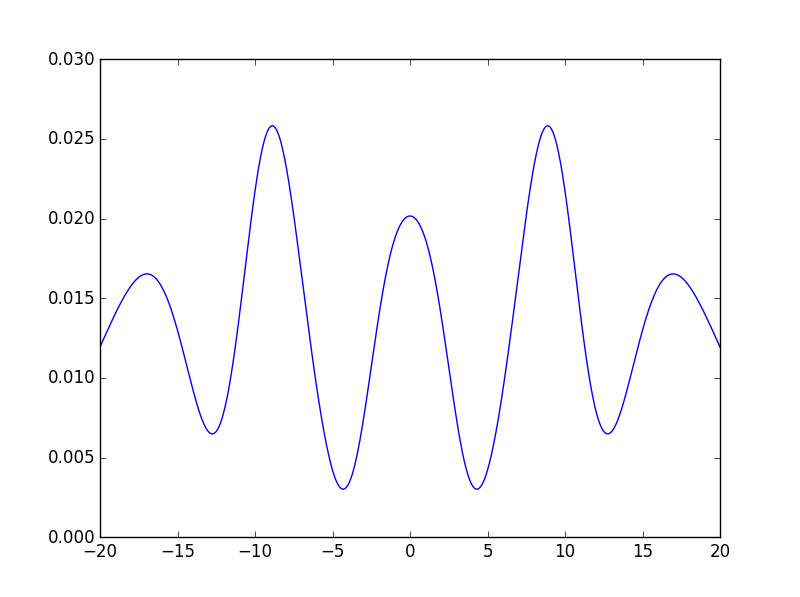
\includegraphics[scale=0.45]{figure_2.png}
	\caption{Intensity profile of linear array of 4 antennae}
\end{figure}

\subsection{Discussion}
Now we have 4 antenna sources, arrange in a linear array. Here we get this radiation pattern by the contribution of all the antenna sources in the array. We get different lobes because of interference, spherical waves coming from each individual antenna source where arrive in phase, they add together (constructive interference) to enhance the intensity and where they arrive out of phase, with the peak of one coinciding with the another, the waves cancel (destructive interference) reducing the intensity in that direction.

\subsection{Managing Phase}

Fig. (1.2) shows a plot between distance and intensity, for four antenna sources arrange in a linear array. Now, by introducing and managing phase among them we can steer the beam as:

\begin{figure}[!h]
	\centering	
	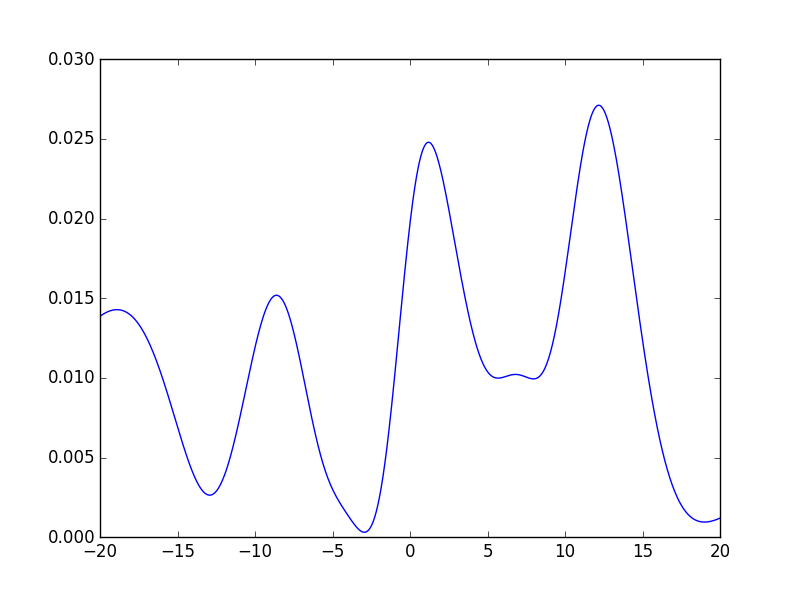
\includegraphics[scale=0.45]{figure_3.png}
	\caption{Intensity profile of linear array of 4 antennae}
\end{figure}

\begin{figure}[!h]
	\centering	
	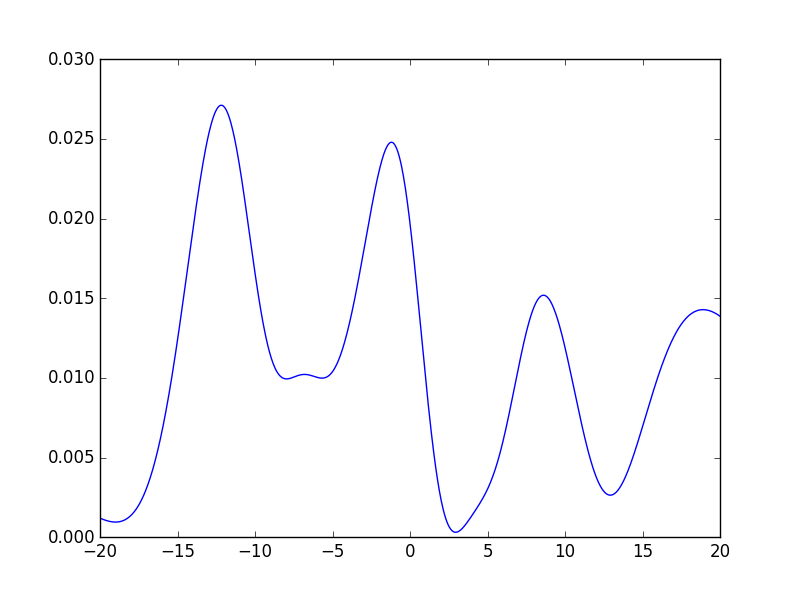
\includegraphics[scale=0.45]{figure_4.png}
	\caption{Intensity profile of linear array of 4 antennae}
\end{figure}

\subsubsection{Discussion}
These are the radiation patterns of antenna sources, by not only introducing fig. (4.2) but managing phase among them, consists of a strong steered beam in one direction which is emitted perpendicular to the plane of the antenna sources, plus a series of weaker beams, usually representing residual radiation in unwanted directions and can not participate in beam formation.

\section{Conclusion}
Fig. (4.3) and (4.4) shows that by introducing and managing phase among multiple antenna sources, we can steer the beam formed by the interference of all the radiations coming from each individual antenna source.

we can form a better and narrow beam with higher intensity by using number of antenna sources with correct phase relation.
